\begin{figure}
    \begin{center}
    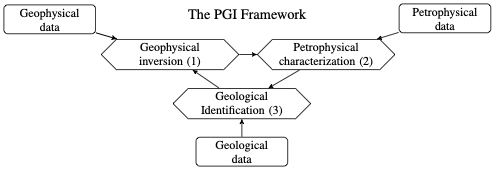
\includegraphics[width=0.75\textwidth]{figures/genererate-pgi-framework-figure.png}
    \end{center}
\caption{
    The PGI framework (modified from \citet{Astic2019}) is composed of three interlocked inverse problems (diamond nodes) over the geophysical, petrophysical, and geological information (represented by the rectangular nodes).
}
\label{fig:pgi-framework}
\end{figure}
